\documentclass[12pt]{article}

% This first part of the file is called the PREAMBLE. It includes
% customizations and command definitions. The preamble is everything
% between \documentclass and \begin{document}.

\usepackage[margin=1in]{geometry}  % set the margins to 1in on all sides
\usepackage{graphicx}              % to include figures
\usepackage{amsmath}               % great math stuff
\usepackage{amsfonts}              % for blackboard bold, etc
\usepackage{amsthm}                % better theorem environments
\usepackage{amssymb} 
\usepackage{mathptmx}
\usepackage{enumerate}
\usepackage{listings}
\usepackage{xcolor}
\usepackage{forest}
\usepackage{tabularx}  

% various theorems, numbered by section

\newtheorem{thm}{Theorem}[section]
\newtheorem{lem}[thm]{Lemma}
\newtheorem{prop}[thm]{Proposition}
\newtheorem{cor}[thm]{Corollary}
\newtheorem{conj}[thm]{Conjecture}
\newtheorem{mydef}[thm]{Definition}
\lstset{
	basicstyle          =   \sffamily,          
	keywordstyle        =   \bfseries,          
	commentstyle        =   \rmfamily\itshape,  
	stringstyle         =   \ttfamily,  
	flexiblecolumns,                
	numbers             =   left,   
	showspaces          =   false,  
	numberstyle         =   \fontsize{5}{skip},    
	showstringspaces    =   false,
	captionpos          =   t,      
	frame               =   lrtb,   
}

\lstdefinestyle{cpp}{
	language        =   cpp, 
	basicstyle      =   \fontsize{5}{skip},
	numberstyle     =   \fontsize{5}{skip},
	keywordstyle    =   \color{blue},
	keywordstyle    =   [2] \color{teal},
	stringstyle     =   \color{magenta},
	commentstyle    =   \color{red}\ttfamily,
	breaklines      =   true,   
	columns         =   fixed,  
	basewidth       =   0.5em,
}
\begin{document}


\title{ CSE 102 Spring 2021\\
	Homework Assignment 7}

\author{Jaden Liu \\ 
University of California at Santa Cruz\\
Santa Cruz, CA 95064 USA }

\maketitle


\section{HW7} 
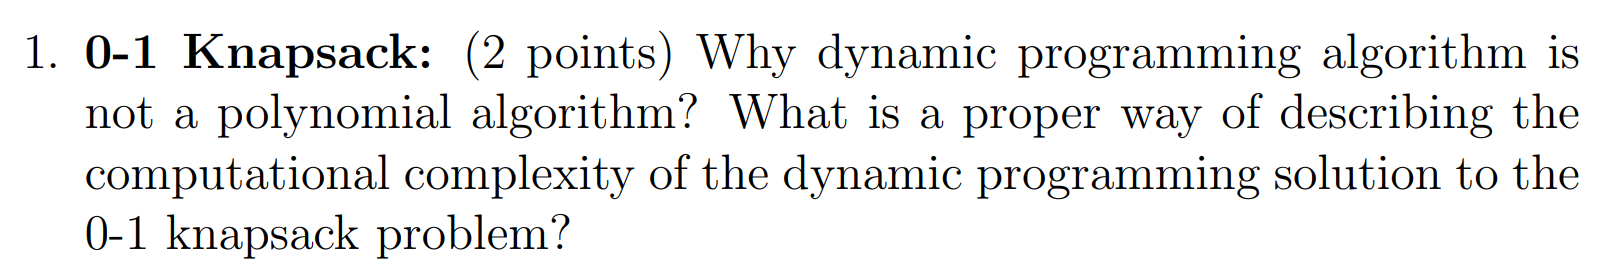
\includegraphics[scale=0.25]{1.png}
\begin{proof}[Solution]
	In the dynamic programming algorithm, we need to fill up a table with n*W size. Therefore the time complexity is O(nW). Since the input size = $logw_1+logv_1+logw_2+logv_2 +...+logw_n+logv_n+logW = nlowW + nlogV$, and V can be accounted for the in the constant term. Thus, the input size = nlogW, which means the runtime is exponential in the input length.\cite{mark}
\end{proof}
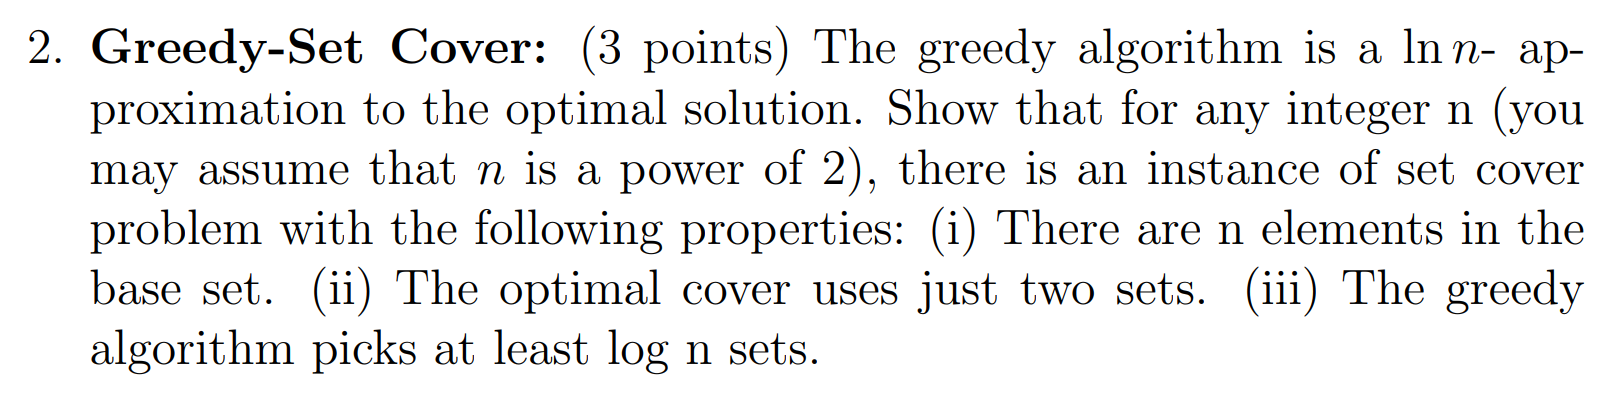
\includegraphics[scale=0.25]{2.png}
\begin{proof}
	I. Since $n_t\le n_0(1-(\frac{1}{k})^t)<ne^{-t/k}$, $n_t$ is strictly less than $ne^{-lnn}=1$ at $t=klnn$, which means no elements remain to be covered. Thus there are n elements in the base case.\\
	II. Just purposedly give a set that only needs two set covering the whole set.\\
	III. Since we have proved that $n_t\le n_0(1-(\frac{1}{k})^t)<ne^{-t/k}$, then the ratio between the optimal solution and greedy algorithm will never be greater than log n sets.
\end{proof}
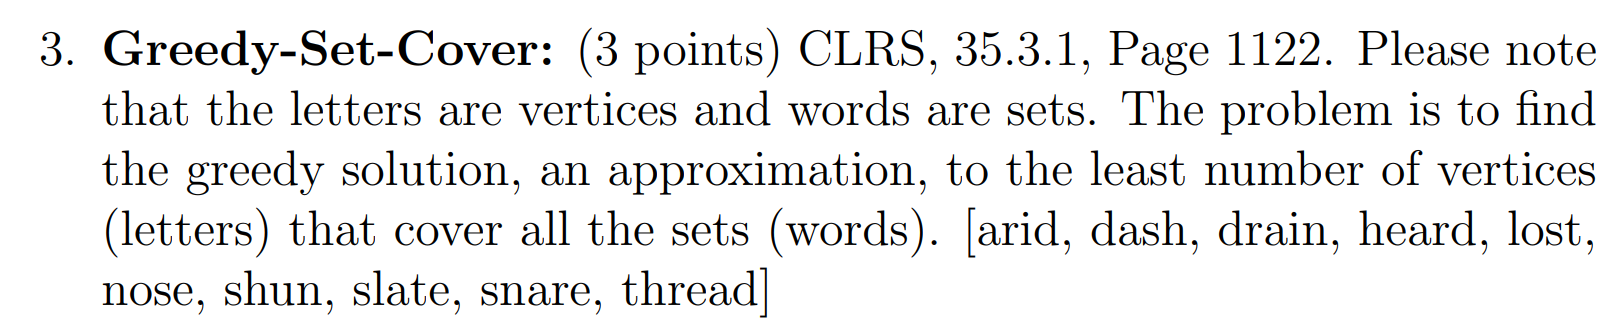
\includegraphics[scale=0.25]{3.png}
\begin{proof}
	First we find thread(6 letters), then shun(4 letters), lost(2 letters) and drain(1 letters).
\end{proof}
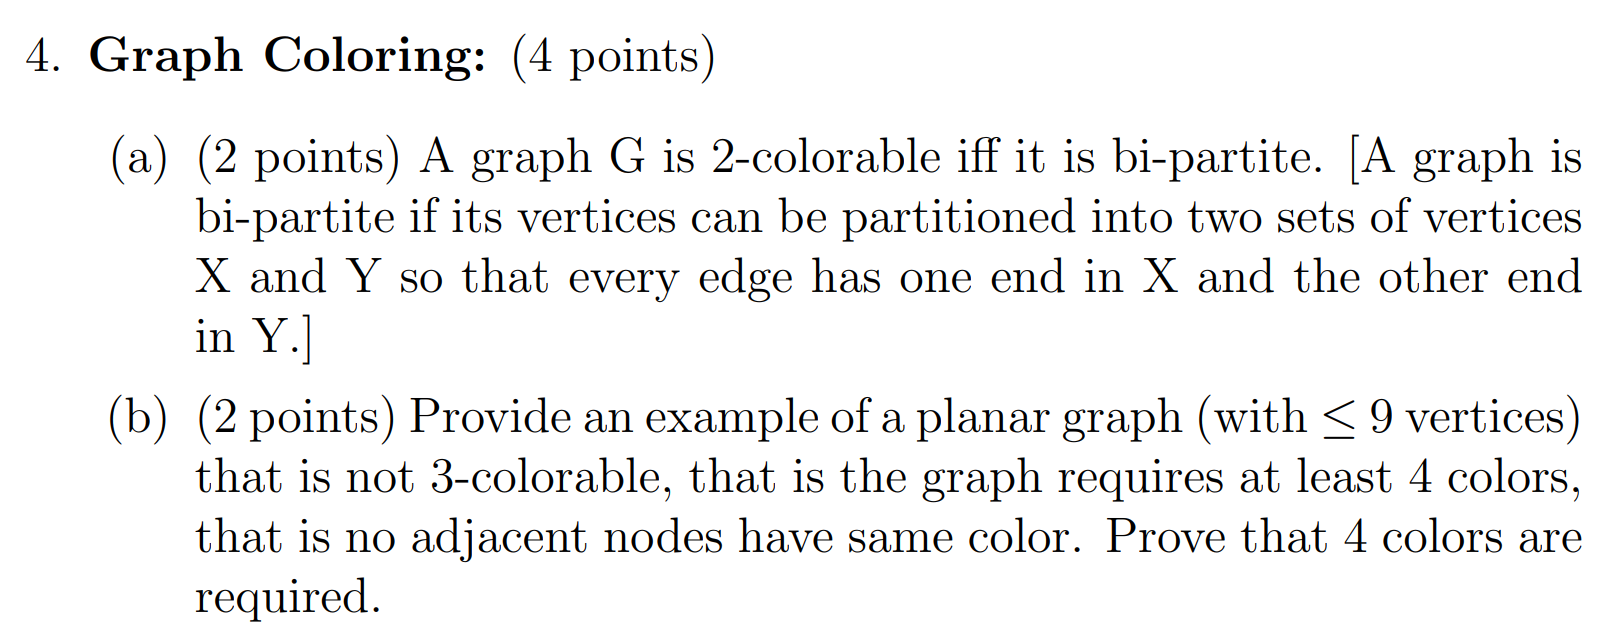
\includegraphics[scale=0.25]{4.png}
\begin{proof}
	a):Let G be a 2-colorable graph, which means we can color every vertex either red or blue,
	and no edge will have both endpoints colored the same color. Let A denote the subset of vertices
	colored red, and let B denote the subset of vertices colored blue. Since all vertices of A are red, there are no edges within A, and similarly for B. This implies that every edge has one endpoint in A and the other in B, which means G is bipartite.\cite{pdf}
	
	Conversely, suppose G is bipartite, that is, we can partition the vertices into two subsets V1, V2 every edge has one endpoint in V1 and the other in V2. Then coloring every vertex of V1 red and every vertex of V2 blue yields a valid coloring, so G is 2-colorable.
\end{proof}
\begin{proof}
	b): 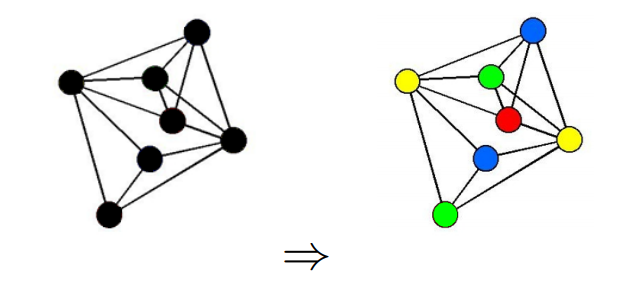
\includegraphics[scale=0.22]{4_2.png} \cite{graph}\\
	In this graph, we can consider the red dot as the center dot. Consider the four point on the left top. They connected each other, so we needs at least 4 colors to represent the graph.
\end{proof}
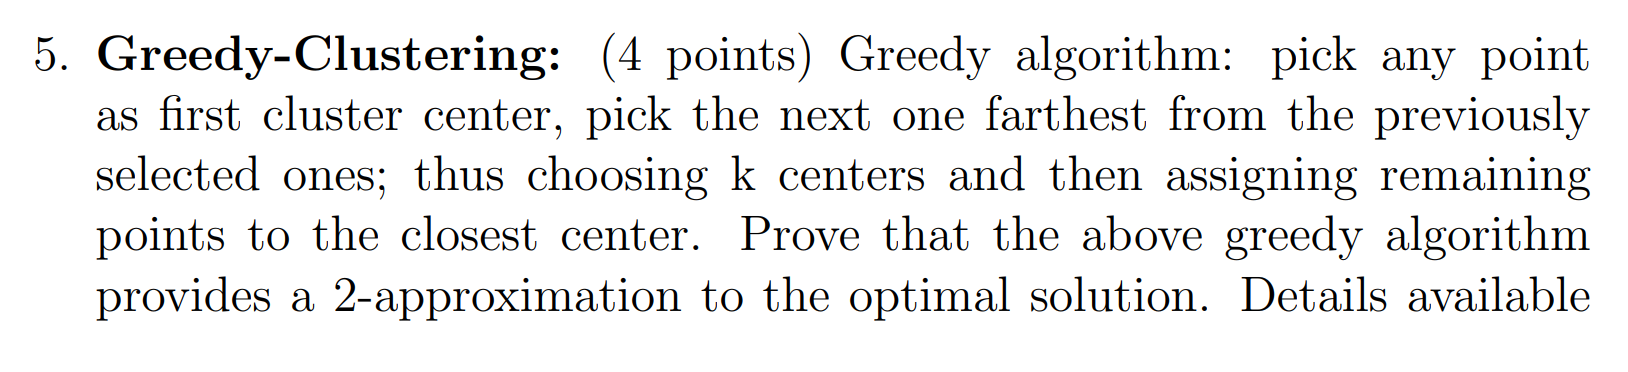
\includegraphics[scale=0.25]{5.png}
\begin{proof}
	Let $x \in X$ be the point farthest from $u_1, . . . , u_k$ (in other words the
	next center we would have chosen, if we wanted $k + 1$ of them), and let $r$ be its distance to its closest center. Then every point in X must be within distance $r$ of its cluster center. By the triangle inequality, this means that every cluster has diameter at most $2r$
\end{proof}
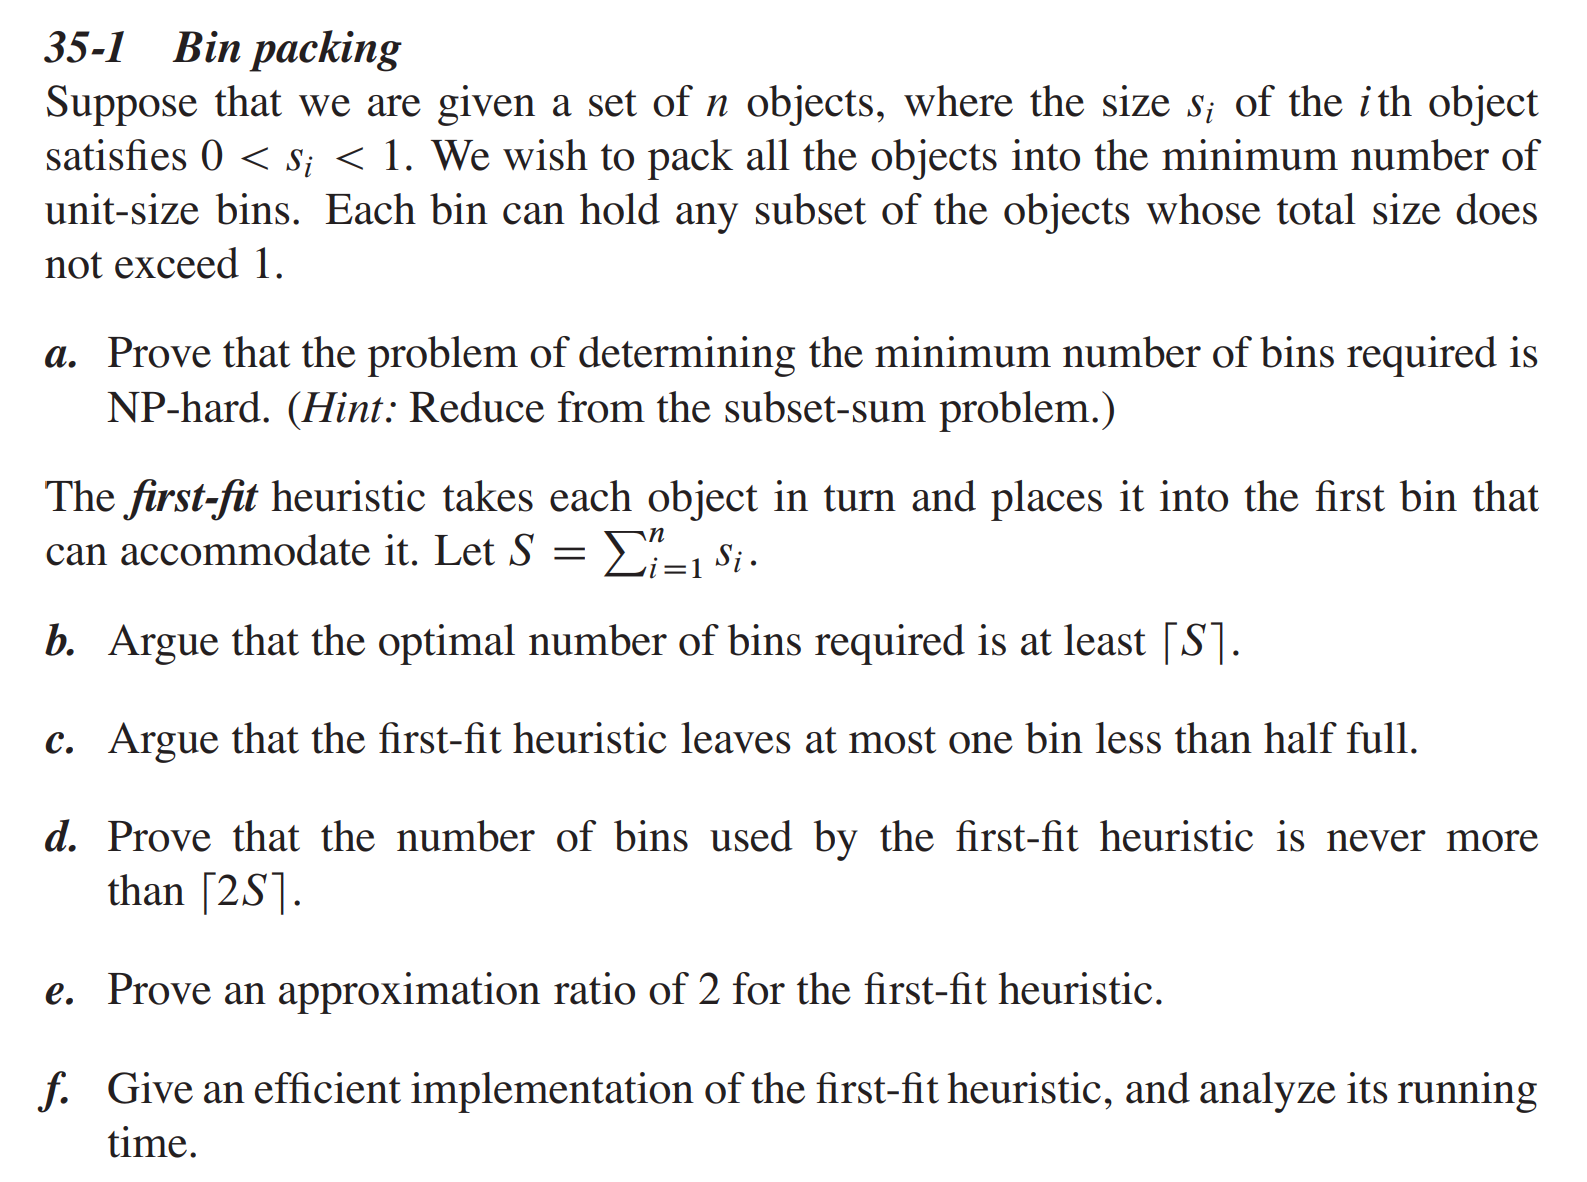
\includegraphics[scale=0.25]{6.png}
\begin{proof}
	b): Assume the we can add partial of the element, then the total bin we need is $\lceil S/1\rceil$. Hence the optimal is at least $\lceil S\rceil$.\\
	c): If there is more than 1 bin that is half full, then we can combine these bin together. Thus, generating a contradiction, which proves that at most 1 half full bin.\\
	d,e): $OPT \ge \sum_{i=1}^{n}a_i > \frac{m-1}{2}$, thus $2OPT >m$\\
	f): Given a object in the list, find if it can be put into the present bin, otherwise put into the next bin(or create a new bin), repeat this process until the end of object list. The running time is $O(n^2)$ in the worst case.
\end{proof}
\begin{thebibliography}{mark}
	\bibitem{mark} Mark Gritter, https://www.quora.com/What-is-a-proper-explanation-of-how-the-dynamic-programming-knapsack-problem-is-not-polynomial-but-pseudo-polynomial
	\bibitem{graph} https://stepik.org/lesson/390640/step/3
	\bibitem{pdf} https://courses.cs.duke.edu//spring19/compsci230/Notes/lecture15.pdf
\end{thebibliography}

\end{document}
